% fig_security_margin.tex
% Security margin (I_thresh / (ε_CT × I_rest)) vs I_rest
% Fixed threshold → margin collapses at high load; adaptive k=0.15 → constant 30×
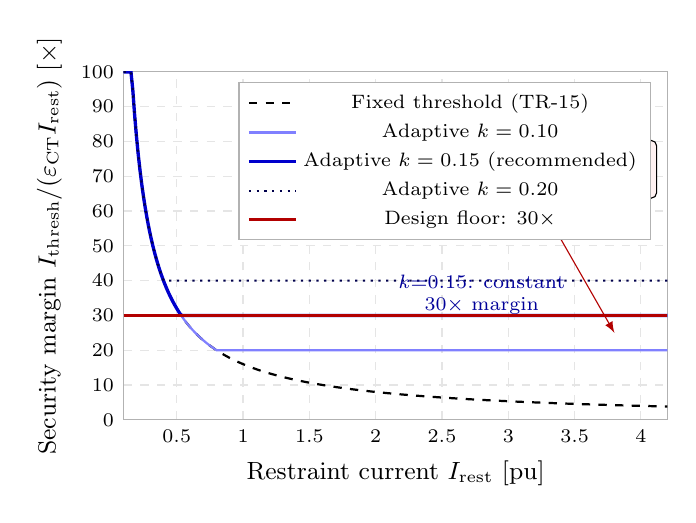
\begin{tikzpicture}
\begin{axis}[
  name        = smgax,
  width       = 0.70\textwidth,
  height      = 6.0cm,
  xlabel      = {Restraint current $I_{\rm rest}$ [pu]},
  ylabel      = {Security margin $I_{\rm thresh} / (\varepsilon_{\rm CT} I_{\rm rest})$ [$\times$]},
  xlabel style= {font=\small},
  ylabel style= {font=\small},
  xmin=0.1, xmax=4.2,
  ymin=0, ymax=100,
  xtick       = {0.5,1,1.5,2,2.5,3,3.5,4},
  ytick       = {0,10,20,30,40,50,60,70,80,90,100},
  xticklabel style={font=\scriptsize},
  yticklabel style={font=\scriptsize},
  legend style={at={(0.97,0.97)}, anchor=north east,
                font=\scriptsize, draw=gray!60, fill=white},
  legend columns=1,
  grid         = major,
  grid style   = {gray!20, dashed},
  tick style   = {draw=none},
  axis line style={gray!60},
  clip=true,
]

% ε_CT = 0.005
% Fixed: margin = 0.08 / (0.005 * x) — collapses as x grows
\addplot[black, thick, dashed, domain=0.1:4.2, samples=300]
  {min(100, 0.08 / (0.005 * x))};
\addlegendentry{Fixed threshold (TR-15)}

% Adaptive k=0.10
\addplot[blue!50, thick, domain=0.1:4.2, samples=300]
  {min(100, max(0.08, 0.10*x) / (0.005 * x))};
\addlegendentry{Adaptive $k=0.10$}

% Adaptive k=0.15 (recommended) — asymptotes to 30×
\addplot[blue!80!black, very thick, domain=0.1:4.2, samples=300]
  {min(100, max(0.08, 0.15*x) / (0.005 * x))};
\addlegendentry{Adaptive $k=0.15$ (recommended)}

% Adaptive k=0.20
\addplot[blue!30!black, thick, dotted, domain=0.1:4.2, samples=300]
  {min(100, max(0.08, 0.20*x) / (0.005 * x))};
\addlegendentry{Adaptive $k=0.20$}

% ---- Minimum margin reference line (30×) ------------------------------------
\addplot[red!70!black, thick, domain=0.1:4.2, samples=2]
  {30};
\addlegendentry{Design floor: 30$\times$}

% ---- Fixed threshold degradation annotation ----------------------------------
\node[draw, fill=red!5, rounded corners=2pt, font=\scriptsize, align=center]
  at (axis cs:3.0, 72)
  {Fixed threshold:\\margin $\to$ 5$\times$ at $I_{\rm rest}=4$\,pu};
\draw[-latex, red!70!black]
  (axis cs:3.2, 65) -- (axis cs:3.8, 25);

% ---- Adaptive flat region annotation ----------------------------------------
\node[font=\scriptsize, blue!60!black, align=center]
  at (axis cs:2.8, 36)
  {$k{=}0.15$: constant\\30$\times$ margin};

\end{axis}
\end{tikzpicture}
